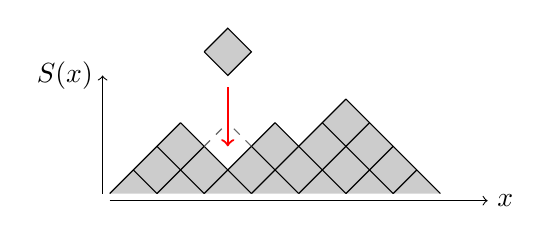
\begin{tikzpicture}[scale = .3]
\draw[->] (0, -.3) -- (16,-.3) node[right]{$x$};
\draw[->] (-.3,0) -- (-.3,5) node[left]{$S(x)$};
\fill[black!20] (0,0) -- (3,3) -- (5,1) -- (7,3) -- (8,2) --
				(10,4) -- (14,0) ;
\draw (0,0) -- (3,3);
\draw (2,0) -- (4,2);
\draw (4,0) -- (7,3);
\draw (6,0) -- (10,4);
\draw (8,0) -- (11,3);
\draw (10,0) -- (12,2);
\draw (12,0) -- (13,1);
\draw (2,0) -- (1,1);
\draw (4,0) -- (2,2);
\draw (6,0) -- (3,3);
\draw (8,0) -- (6,2);
\draw (10,0) -- (7,3);
\draw (12,0) -- (9,3);
\draw (14,0) -- (10,4);
\draw[dashed, black!60]  (4,2) -- (5,3);
\draw[dashed, black!60]  (6,2) -- (5,3);

\draw[fill=black!20] (4,6) -- (5,5) -- (6,6) -- (5,7) -- (4,6);
\draw[thick, ->, red] (5,4.5) -- (5,2);
\end{tikzpicture}
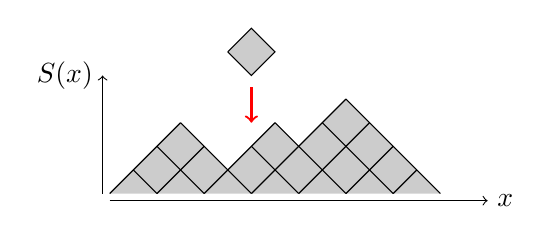
\begin{tikzpicture}[scale = .3, cross/.style={path picture={ 
		\draw[black]
		(path picture bounding box.south east) -- (path picture bounding box.north west) (path picture bounding box.south west) -- (path picture bounding box.north east);
}}]

\draw[->] (0, -.3) -- (16,-.3) node[right]{$x$};
\draw[->] (-.3,0) -- (-.3,5) node[left]{$S(x)$};
\fill[black!20] (0,0) -- (3,3) -- (5,1) -- (7,3) -- (8,2) --
(10,4) -- (14,0) ;
\draw (0,0) -- (3,3);
\draw (2,0) -- (4,2);
\draw (4,0) -- (7,3);
\draw (6,0) -- (10,4);
\draw (8,0) -- (11,3);
\draw (10,0) -- (12,2);
\draw (12,0) -- (13,1);
\draw (2,0) -- (1,1);
\draw (4,0) -- (2,2);
\draw (6,0) -- (3,3);
\draw (8,0) -- (6,2);
\draw (10,0) -- (7,3);
\draw (12,0) -- (9,3);
\draw (14,0) -- (10,4);
%\draw[dashed, black!60]  (5,3) -- (6,4);
%\draw[dashed, black!60]  (7,3) -- (6,4);
%\draw[dashed, black!60]  (6,2) -- (5,3);

\draw[fill=black!20] (5,6) -- (6,5) -- (7,6) -- (6,7) -- (5,6);
\draw[thick, ->, red] (6,4.5) -- (6,3);
%\node [draw,circle,cross,minimum width=1](B) at (6,3.5){}; 
\end{tikzpicture}
